
\documentclass[12pt]{article}
\usepackage[utf8]{inputenc}
\usepackage[spanish]{babel}
\usepackage{amsmath}
\usepackage{geometry}
\usepackage{graphicx}
\usepackage{listings}
\usepackage{color}
\geometry{margin=2.5cm}

\title{Paralelización en CUDA: Transformada de Fourier Discreta y Continua}
\author{Jesús Losada Arauzo}
\date{\today}

\begin{document}

\maketitle

\section*{Resumen}

En este informe se analiza la paralelización mediante CUDA de la Transformada de Fourier Discreta (DFT) y versiones continuas con integración numérica. El objetivo es medir el rendimiento frente a la versión secuencial utilizando diferentes técnicas de integración: suma de rectángulos, trapecios y método de Simpson. Se emplea memoria unificada y eventos CUDA para una gestión sencilla de datos y tiempos.

\section*{Paralelización en CUDA}

El programa implementa varios \textit{kernels} CUDA, uno para cada versión de la transformada:

\begin{itemize}
    \item \textbf{DFT}: versión discreta clásica.
    \item \textbf{CFT}: versión continua básica, usando suma directa.
    \item \textbf{CFT\_Trapecio} y \textbf{CFT\_Simpson}: integración continua por métodos numéricos.
\end{itemize}

Se utiliza una distribución fija de hilos: \texttt{BLOCK\_SIZE = 256} y \texttt{NUM\_BLOCKS = 10}. Cada hilo se encarga de calcular una componente del vector de Fourier (una frecuencia). Internamente, el hilo hace un bucle que suma o integra la función con el método correspondiente.

\subsection*{Distribución del trabajo}

Cada hilo CUDA calcula un índice global:

\[
\texttt{i = blockIdx.x * blockDim.x + threadIdx.x}
\]

Con ese índice se decide si se procesa la componente \( i \) del vector de salida. De este modo, la carga de trabajo se distribuye automáticamente entre los hilos, permitiendo ejecutar en paralelo todos los valores de la transformada.

\subsection*{Medición de tiempo}

El tiempo se mide mediante \texttt{cudaEventRecord}, lo cual permite medir con precisión únicamente la ejecución del kernel (sin contar asignaciones ni E/S). El resultado se almacena en archivos para su posterior graficado.

\section*{Resultados obtenidos}

Las siguientes gráficas muestran los tiempos medidos en milisegundos para distintos tamaños de muestra. Se comparan versiones secuenciales y paralelas.

\begin{itemize}
    \item Para muestras pequeñas, CUDA tiene cierta penalización inicial.
    \item A partir de cierto tamaño, la versión paralela supera ampliamente a la secuencial.
\end{itemize}

\begin{figure}[h]
    \centering
    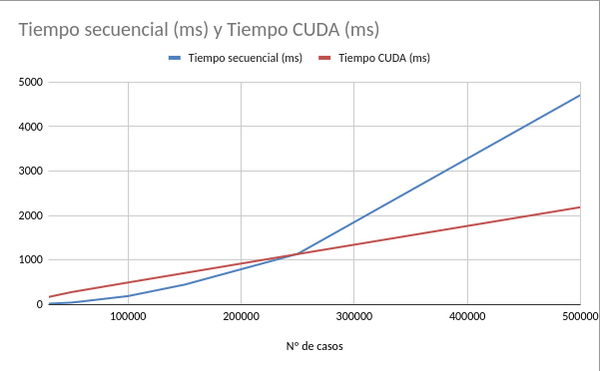
\includegraphics[width=0.8\textwidth]{captura1.png}
    \caption{Tiempo de ejecución - DFT (Transformada Discreta)}
\end{figure}

\begin{figure}[h]
    \centering
    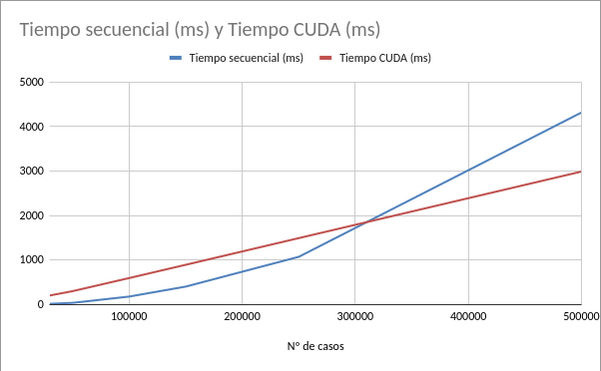
\includegraphics[width=0.8\textwidth]{captura2.png}
    \caption{Tiempo de ejecución - Suma de Rectángulos}
\end{figure}

\begin{figure}[h]
    \centering
    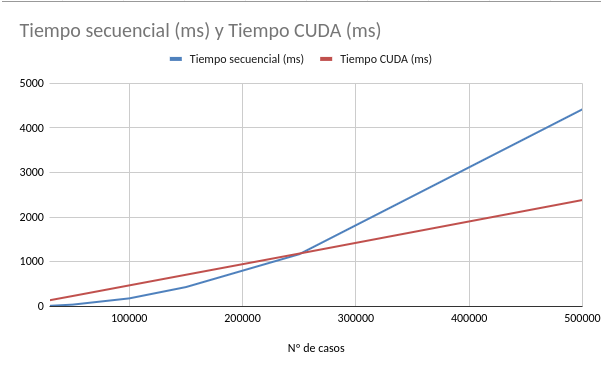
\includegraphics[width=0.8\textwidth]{captura3.png}
    \caption{Tiempo de ejecución - Método del Trapecio}
\end{figure}

\begin{figure}[h]
    \centering
    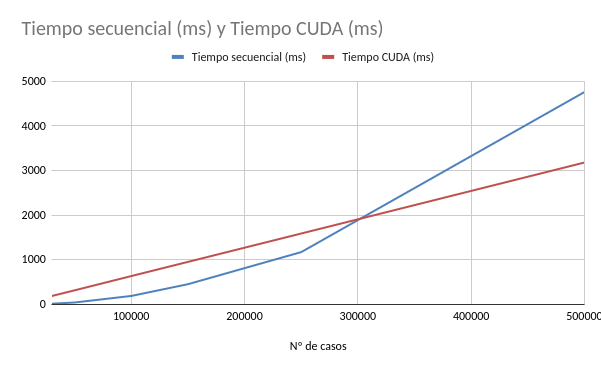
\includegraphics[width=0.8\textwidth]{captura4.png}
    \caption{Tiempo de ejecución - Método de Simpson}
\end{figure}

\newpage

\section*{Código CUDA resumido}

\begin{lstlisting}[language=C++, basicstyle=\ttfamily\small, frame=single]
__global__ void DFT(cuDoubleComplex *Fourier, const double *muestras, int N){
    int i = blockIdx.x * blockDim.x + threadIdx.x;
    if (i < N){
        cuDoubleComplex sum = make_cuDoubleComplex(0.0, 0.0);
        for (int j = 0; j < N; j++){
            double angle = -2.0 * PI * i * j / N;
            cuDoubleComplex term = make_cuDoubleComplex(muestras[j]*cos(angle),
                                                        muestras[j]*sin(angle));
            sum = cuCadd(sum, term);
        }
        Fourier[i] = sum;
    }
}
\end{lstlisting}

\section*{Conclusión}

Gracias a la paralelización en CUDA, se consigue una mejora notable en el rendimiento del cálculo de transformadas de Fourier a gran escala. Aunque la inicialización de la GPU introduce cierta latencia, para volúmenes de datos grandes la ejecución en GPU resulta significativamente más rápida que la versión secuencial.

\end{document}
